\chapter[Contexto Zenit Aerospace]{Contexto Zenit Aerospace}
A Zenit Aerospace é uma empresa júnior, da Univerdade de Brasília - Campus gama. A empresa é mantida pelos próprios alunos, estes são principalmente do curso de aeroespacial. 
\begin{itemize}
\item \textbf{Objetivos:} o objetivo principal da Zenit é de proporcionar aos estudantes que participam da iniciativa, o contato profissional com as áreas do conhecimentos da engenharia aeroespacial. Provocar o interesse da sociedade brasileira na área de operação da empresa, por meio do desenvolvimentos de projetos para o mercado, formentando o sugimento de uma cultura no setor. 
\item\textbf{Missão:} prover aos membros a oportunidade de durante a formação ter contato com o universo profissional da Engenharia Aeroespacial e motivá-los para novas ideias e transformar essas em realidade \cite{regimentoZenit}.
\end{itemize}
\section{Organização da empresa}
Atualmente a Zenit Aerospace é dividida em dois tipos de funcionários: gestores e assessores. Os cargos de gestão são delegados a estudantes que são incorporados a empresa, cuja função é coordenar, gerir, controlar, uma das cinco diretorias ou a presidência da empresa. Aqueles que não estão no cargo de gerência são assessores, em que a responsabilidade é assessorar, auxiliar, dar suporte aos gestores. Ressalta-se que a participação no desenvolvimento de projetos não é restrita.
\begin{figure}[h]
	\centering
	\label{zenitOrganograma}
    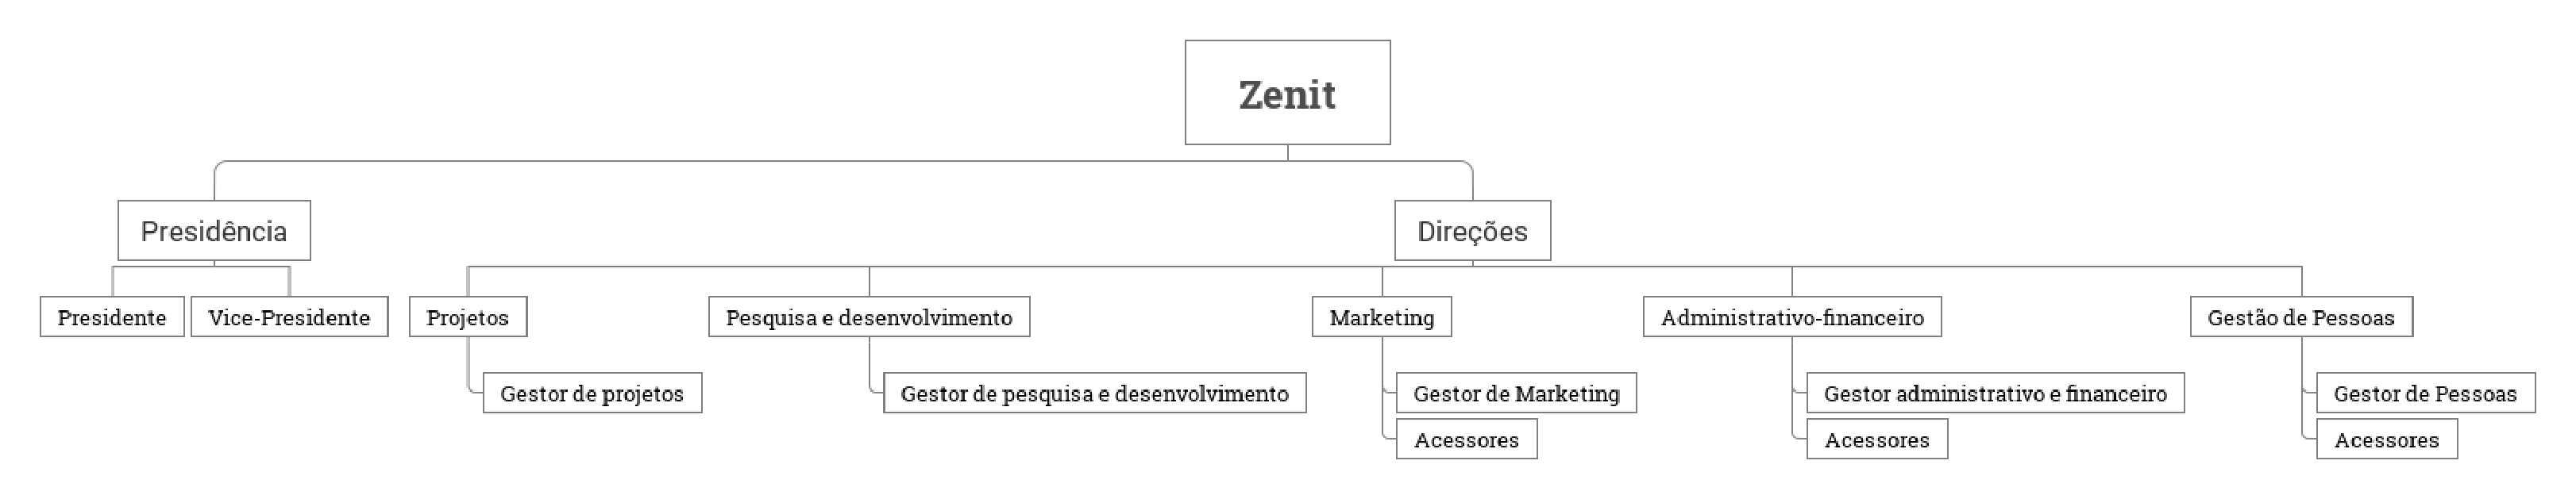
\includegraphics[keepaspectratio=true,scale=0.3]{figuras/zenitOrganograma.eps}
	\caption{Organograma da empresa Zenit Aerospace}
\end{figure}
As demais direções executivas são: Presidência, Gestão de Pessoas, Marketing, Administrativo-financeiro, Projeto e Pesquisa e desenvolvimento.
A presidência, é responsável por aprovar admissão ou demissão de membros, decidir responsáveis para cada etapa dos projetos, garantir o funcionamento das demais diretorias entre outros \cite{regimentoZenit}. 
A direção de pessoas é responsável por supervisionar a atualização do banco de dados de membros da empresa, prover a motivação dos membros mediante políticas de reconhecimento, emissão de certificados da participação dos membros em projetos, auxiliar no planejamento de treinamentos, seleção de membros para os projetos \cite{regimentoZenit}. 
A direção de projetos é responsável por gerir os projetos, trabalhos, demandas para a empresa. Esta área determinará a quantidade de pessoas a serem alocadas, as capacidades técnicas necessárias e juntamente com a direção de pessoas, quais funcionários possuem os requisitos para preencher a vaga no projeto \cite{regimentoZenit}.

\section[Descrição do problema]{Descrição do problema}\label{descricaoProblema}

O gestor de pessoas é responsável por organizar os dados dos funcionários da Zenit com relação a sua capacitação e seus dados pessoais. A atual forma para manter os dados, não atende a expectativa do gestor de pessoas, pois dificulta a utilização destes para o desempenho de suas atividades que necessite da informação dos funcionários. Há uma planilha online do Google Drive no qual todos os dados pessoais dos funcionários ficam registrados, porém não há o registro da capacitação de cada funcionário. Todos os membros recebem acesso, mas somente  o gestor de pessoas e o presidente organizacional tem autorização de modificar algum dado. Caso algum funcionário saia da empresa, é responsabilidade do gestor de pessoas remover os dados do ex funcionário, assim como o acesso as informações dos demais funcionários.

A metodologia atual adotada pela empresa, uso de planilhas,  não atende as principais necessidades  da área de gerenciamento de pessoas, que é conseguir fazer acompanhamento das habilidades técnicas e experiências, e determinar com base nos dados de qualificação de cada membro quais são as atividades recomendáveis para ele desempenhar. Além disso, a área de gestão de pessoas da empresa está implementando os processos para o gerenciamento dos funcionários, tais como: meritocracia para funcionários, bonificações, acompanhamento das atividades dos membros da empresa.

Na metodologia atual adotada pela empresa, quando há a demanda de uma atividade, há uma lista que circula entre todos os membros da empresa na qual conterá os nomes dos integrantes interessados em participar, como não há o acompanhamento das competências dos funcionários é adicionado um questionário para obter tais informações caso seja necessário. Em seguida o presidente organizacional e o gestor de pessoas avalia quem são os funcionários adequados para realizar a atividade.


